\documentclass[]{article}
\usepackage{lmodern}
\usepackage{amssymb,amsmath}
\usepackage{ifxetex,ifluatex}
\usepackage{fixltx2e} % provides \textsubscript
\ifnum 0\ifxetex 1\fi\ifluatex 1\fi=0 % if pdftex
  \usepackage[T1]{fontenc}
  \usepackage[utf8]{inputenc}
\else % if luatex or xelatex
  \ifxetex
    \usepackage{mathspec}
  \else
    \usepackage{fontspec}
  \fi
  \defaultfontfeatures{Ligatures=TeX,Scale=MatchLowercase}
\fi
% use upquote if available, for straight quotes in verbatim environments
\IfFileExists{upquote.sty}{\usepackage{upquote}}{}
% use microtype if available
\IfFileExists{microtype.sty}{%
\usepackage{microtype}
\UseMicrotypeSet[protrusion]{basicmath} % disable protrusion for tt fonts
}{}
\usepackage[margin=1in]{geometry}
\usepackage{hyperref}
\hypersetup{unicode=true,
            pdftitle={Body size trends in Neogene tortoises},
            pdfborder={0 0 0},
            breaklinks=true}
\urlstyle{same}  % don't use monospace font for urls
\usepackage{color}
\usepackage{fancyvrb}
\newcommand{\VerbBar}{|}
\newcommand{\VERB}{\Verb[commandchars=\\\{\}]}
\DefineVerbatimEnvironment{Highlighting}{Verbatim}{commandchars=\\\{\}}
% Add ',fontsize=\small' for more characters per line
\usepackage{framed}
\definecolor{shadecolor}{RGB}{248,248,248}
\newenvironment{Shaded}{\begin{snugshade}}{\end{snugshade}}
\newcommand{\KeywordTok}[1]{\textcolor[rgb]{0.13,0.29,0.53}{\textbf{{#1}}}}
\newcommand{\DataTypeTok}[1]{\textcolor[rgb]{0.13,0.29,0.53}{{#1}}}
\newcommand{\DecValTok}[1]{\textcolor[rgb]{0.00,0.00,0.81}{{#1}}}
\newcommand{\BaseNTok}[1]{\textcolor[rgb]{0.00,0.00,0.81}{{#1}}}
\newcommand{\FloatTok}[1]{\textcolor[rgb]{0.00,0.00,0.81}{{#1}}}
\newcommand{\ConstantTok}[1]{\textcolor[rgb]{0.00,0.00,0.00}{{#1}}}
\newcommand{\CharTok}[1]{\textcolor[rgb]{0.31,0.60,0.02}{{#1}}}
\newcommand{\SpecialCharTok}[1]{\textcolor[rgb]{0.00,0.00,0.00}{{#1}}}
\newcommand{\StringTok}[1]{\textcolor[rgb]{0.31,0.60,0.02}{{#1}}}
\newcommand{\VerbatimStringTok}[1]{\textcolor[rgb]{0.31,0.60,0.02}{{#1}}}
\newcommand{\SpecialStringTok}[1]{\textcolor[rgb]{0.31,0.60,0.02}{{#1}}}
\newcommand{\ImportTok}[1]{{#1}}
\newcommand{\CommentTok}[1]{\textcolor[rgb]{0.56,0.35,0.01}{\textit{{#1}}}}
\newcommand{\DocumentationTok}[1]{\textcolor[rgb]{0.56,0.35,0.01}{\textbf{\textit{{#1}}}}}
\newcommand{\AnnotationTok}[1]{\textcolor[rgb]{0.56,0.35,0.01}{\textbf{\textit{{#1}}}}}
\newcommand{\CommentVarTok}[1]{\textcolor[rgb]{0.56,0.35,0.01}{\textbf{\textit{{#1}}}}}
\newcommand{\OtherTok}[1]{\textcolor[rgb]{0.56,0.35,0.01}{{#1}}}
\newcommand{\FunctionTok}[1]{\textcolor[rgb]{0.00,0.00,0.00}{{#1}}}
\newcommand{\VariableTok}[1]{\textcolor[rgb]{0.00,0.00,0.00}{{#1}}}
\newcommand{\ControlFlowTok}[1]{\textcolor[rgb]{0.13,0.29,0.53}{\textbf{{#1}}}}
\newcommand{\OperatorTok}[1]{\textcolor[rgb]{0.81,0.36,0.00}{\textbf{{#1}}}}
\newcommand{\BuiltInTok}[1]{{#1}}
\newcommand{\ExtensionTok}[1]{{#1}}
\newcommand{\PreprocessorTok}[1]{\textcolor[rgb]{0.56,0.35,0.01}{\textit{{#1}}}}
\newcommand{\AttributeTok}[1]{\textcolor[rgb]{0.77,0.63,0.00}{{#1}}}
\newcommand{\RegionMarkerTok}[1]{{#1}}
\newcommand{\InformationTok}[1]{\textcolor[rgb]{0.56,0.35,0.01}{\textbf{\textit{{#1}}}}}
\newcommand{\WarningTok}[1]{\textcolor[rgb]{0.56,0.35,0.01}{\textbf{\textit{{#1}}}}}
\newcommand{\AlertTok}[1]{\textcolor[rgb]{0.94,0.16,0.16}{{#1}}}
\newcommand{\ErrorTok}[1]{\textcolor[rgb]{0.64,0.00,0.00}{\textbf{{#1}}}}
\newcommand{\NormalTok}[1]{{#1}}
\usepackage{graphicx,grffile}
\makeatletter
\def\maxwidth{\ifdim\Gin@nat@width>\linewidth\linewidth\else\Gin@nat@width\fi}
\def\maxheight{\ifdim\Gin@nat@height>\textheight\textheight\else\Gin@nat@height\fi}
\makeatother
% Scale images if necessary, so that they will not overflow the page
% margins by default, and it is still possible to overwrite the defaults
% using explicit options in \includegraphics[width, height, ...]{}
\setkeys{Gin}{width=\maxwidth,height=\maxheight,keepaspectratio}
\IfFileExists{parskip.sty}{%
\usepackage{parskip}
}{% else
\setlength{\parindent}{0pt}
\setlength{\parskip}{6pt plus 2pt minus 1pt}
}
\setlength{\emergencystretch}{3em}  % prevent overfull lines
\providecommand{\tightlist}{%
  \setlength{\itemsep}{0pt}\setlength{\parskip}{0pt}}
\setcounter{secnumdepth}{0}
% Redefines (sub)paragraphs to behave more like sections
\ifx\paragraph\undefined\else
\let\oldparagraph\paragraph
\renewcommand{\paragraph}[1]{\oldparagraph{#1}\mbox{}}
\fi
\ifx\subparagraph\undefined\else
\let\oldsubparagraph\subparagraph
\renewcommand{\subparagraph}[1]{\oldsubparagraph{#1}\mbox{}}
\fi

%%% Use protect on footnotes to avoid problems with footnotes in titles
\let\rmarkdownfootnote\footnote%
\def\footnote{\protect\rmarkdownfootnote}

%%% Change title format to be more compact
\usepackage{titling}

% Create subtitle command for use in maketitle
\newcommand{\subtitle}[1]{
  \posttitle{
    \begin{center}\large#1\end{center}
    }
}

\setlength{\droptitle}{-2em}
  \title{Body size trends in Neogene tortoises}
  \pretitle{\vspace{\droptitle}\centering\huge}
  \posttitle{\par}
  \author{}
  \preauthor{}\postauthor{}
  \date{}
  \predate{}\postdate{}


\begin{document}
\maketitle

\section{30.05.2017}\label{section}

Test paleoTS with Fossil Checklist data (but is probably of no use,
because they report average body sizes (means, median, something else?
what are the respective sample size? maybe ask the authors!?), so this
is just for playing around).

Raw data:

\begin{Shaded}
\begin{Highlighting}[]
\KeywordTok{library}\NormalTok{(paleoTS)}
\CommentTok{#setwd("//naturkundemuseum-berlin.de/MuseumDFSRoot/Benutzer/Julia.Joos/Eigene Dateien/MA")}
\NormalTok{test<-}\KeywordTok{read.csv}\NormalTok{(}\StringTok{"test26.5.csv"}\NormalTok{, }\DataTypeTok{sep=}\StringTok{";"}\NormalTok{, }\DataTypeTok{header=}\OtherTok{TRUE}\NormalTok{)}
\NormalTok{test}
\end{Highlighting}
\end{Shaded}

\begin{verbatim}
##                               Taxon Age_min Age_max Age_mean
## 1                Gopherus pertenuis  0.7810  1.8060  1.29350
## 2          Hesperotestudo johnstoni  0.7810  1.8060  1.29350
## 3           Hesperotestudo oelrichi  0.7810  1.8060  1.29350
## 4            Hesperotestudo turgida  0.7810  1.8060  1.29350
## 5               Megalochelys margae  0.7810  1.8060  1.29350
## 6             Megalochelys sondaari  0.7810  1.8060  1.29350
## 7         Megalochelys sp. [Flores]  0.7810  1.8060  1.29350
## 8           Megalochelys sp. [Java]  0.7810  1.8060  1.29350
## 9            Psammobates antiquorum  0.7810  1.8060  1.29350
## 10         Testudinidae sp. [China]  0.7810  1.8060  1.29350
## 11            Testudo changshanesis  0.7810  1.8060  1.29350
## 12 Hesperotestudo sp. [El Salvador]  0.7810  1.8060  1.29350
## 13            Aldabrachelys abrupta  0.0000  0.0117  0.00585
## 14        Aldabrachelys grandidieri  0.0000  0.0117  0.00585
## 15           Chelonoidis alburyorum  0.0000  0.0117  0.00585
## 16         Chelonoidis sp. [Caicos]  0.0000  0.0117  0.00585
## 17          Chelonoidis sp. [Turks]  0.0000  0.0117  0.00585
## 18           Titanochelon schafferi  5.3320  7.2460  6.28900
## 19                Chelonoidis elata  1.8060  7.2460  4.52600
## 20              Homopus fenestratus  3.6000  1.8060  2.70300
## 21               Chelonoidis lutzae  0.0117  0.1260  0.06885
## 22         Chelonoidis sombrerensis  0.0117  0.1260  0.06885
## 23        Chelonoidis sp. [Navassa]  0.0117  0.1260  0.06885
## 24                Gopherus donlaloi  0.0117  0.1260  0.06885
## 25         Hesperotestudo equicomes  0.0117  0.1260  0.06885
## 26            Hesperotestudo incisa  0.0117  0.1260  0.06885
## 27               Testudo suttoensis  0.0117  0.1260  0.06885
## 28           Hesperotestudo wilsoni  0.0010  0.1260  0.06350
## 29                  Manouria oyamai  0.0010  0.1260  0.06350
## 30     Chelonoidis sp. [Hispaniola]  0.0010  0.1260  0.06350
## 31             Chelonoidis monensis  0.0000  0.1260  0.06300
## 32       Aldabrachelys laetoliensis  0.1260  3.6000  1.86300
## 33            Centrochelys marocana  0.1260  3.6000  1.86300
## 34           Gopherus sp. [Florida]  0.1260  3.6000  1.86300
## 35         Hesperotestudo campester  0.1260  3.6000  1.86300
## 36            Manouria punjabiensis  0.1260  3.6000  1.86300
## 37               Megalochelys atlas  0.1260  3.6000  1.86300
## 38            Megalochelys cautleyi  0.1260  3.6000  1.86300
## 39     Testudo or Agrionemys ranovi  0.1260  3.6000  1.86300
## 40             Testudo oughlamensis  0.1260  3.6000  1.86300
## 41                Testudo pecorinii  0.1260  3.6000  1.86300
## 42            Testudo transcaucasia  0.1260  3.6000  1.86300
## 43        Titanochelon sp. [Lesvos]  0.1260  3.6000  1.86300
## 44           Centrochelys vulcanica  0.1260  3.6000  1.86300
## 45           Centrochelys burchardi  0.1260  0.7810  0.45350
## 46             Centrochelys robusta  0.1260  0.7810  0.45350
## 47          Hesperotestudo bermudae  0.1260  0.7810  0.45350
## 48        Hesperotestudo mlynarskii  0.1260  0.7810  0.45350
## 49         Hesperotestudo percrassa  0.1260  0.7810  0.45350
## 50              Testudo kenitrensis  0.1260  0.7810  0.45350
## 51              Testudo lunellensis  0.1260  0.7810  0.45350
## 52         Titatochelon sp. [Ibiza]  0.1260  0.7810  0.45350
## 53      Hesperotestudo crassicutata  0.7810  0.0117  0.39635
## 54        Chelonoidis sp. [Curaçao]  0.0117  0.7810  0.39635
## 55            Gopherus laticaudatus  0.0117  0.7810  0.39635
## 56         Megalochelys sp. [Timor]  0.0117  0.7810  0.39635
## 57  Aldabrachelys gigantea daudinii  0.0000  0.0000  0.00000
## 58           Chelonoidis abingdonii  0.0000  0.0000  0.00000
## 59                Chelonoidis nigra  0.0000  0.0000  0.00000
## 60          Chelonoidis phantastica  0.0000  0.0000  0.00000
## 61       Chelonoidis sp. [Santa Fé]  0.0000  0.0000  0.00000
## 62             Chylindrapsis inepta  0.0000  0.0000  0.00000
## 63          Chylindrapsis peltastes  0.0000  0.0000  0.00000
## 64         Chylindrapsis triserrata  0.0000  0.0000  0.00000
## 65             Chylindraspis indica  0.0000  0.0000  0.00000
## 66           Chylindraspis vosmaeri  0.0000  0.0000  0.00000
## 67           Centrochelys atlantica  0.0117  2.5880  1.29985
## 68                 Testudo sellovii  0.0117  2.5880  1.29985
## 69             Chelonoidis cubensis  0.1000  2.5880  1.34400
## 70           Titanochelon gymnesica  1.0000  3.6000  2.30000
## 71              Testudo kalganensis  1.0000  3.6000  2.30000
##                                                     Age CL_mean CL_range n
## 1                                     Early Pleistocene   107.5          1
## 2                                     Early Pleistocene    24.0          1
## 3                                     Early Pleistocene    28.0          1
## 4                                     Early Pleistocene    23.0          1
## 5                                     Early Pleistocene   165.0          1
## 6                                     Early Pleistocene    80.0    80-95 1
## 7                                     Early Pleistocene   120.0  180-200 1
## 8                                     Early Pleistocene   175.0          1
## 9                                     Early Pleistocene    11.0    60-65 1
## 10                                    Early Pleistocene    90.0          1
## 11                                    Early Pleistocene    33.0          1
## 12                            Early to Late Pleistocene   150.0          1
## 13                                        Late Holocene   115.0  180-210 1
## 14                                        Late Holocene   125.0          1
## 15                                        Late Holocene    47.0          1
## 16                                        Late Holocene    75.0          1
## 17                                        Late Holocene    37.5          1
## 18                                         Late Miocene   192.5   90-100 1
## 19                   Late Miocene to Early Pleistocene?   195.0    60-90 1
## 20 Late Neogene; possibly Pliocene to Early Pleistocene     9.0          1
## 21                                     Late Pleistocene    83.0          1
## 22                                     Late Pleistocene    95.0          1
## 23                                     Late Pleistocene    40.0          1
## 24                                     Late Pleistocene    58.0    35-40 1
## 25                                     Late Pleistocene    34.0          1
## 26                                     Late Pleistocene    29.0          1
## 27                                     Late Pleistocene    20.0          1
## 28                   Late Pleistocene to Early Holocene    23.0          1
## 29                   Late Pleistocene to Early Holocene    45.0          1
## 30                  Late Pleistocene to Early Holocene?    60.0          1
## 31                    Late Pleistocene to Late Holocene    50.0    35-40 1
## 32                   Late Pliocene to Early Pleistocene   100.0  105-110 1
## 33                   Late Pliocene to Early Pleistocene   190.0    18-26 1
## 34                   Late Pliocene to Early Pleistocene    22.0          1
## 35                   Late Pliocene to Early Pleistocene   100.0          1
## 36                   Late Pliocene to Early Pleistocene    90.0  120-125 1
## 37                   Late Pliocene to Early Pleistocene   195.0          1
## 38                   Late Pliocene to Early Pleistocene   120.0          1
## 39                   Late Pliocene to Early Pleistocene    20.0          1
## 40                   Late Pliocene to Early Pleistocene    12.0          1
## 41                   Late Pliocene to Early Pleistocene    22.5          1
## 42                   Late Pliocene to Early Pleistocene    15.0          1
## 43                   Late Pliocene to Early Pleistocene   186.0          1
## 44                   Late Pliocene to EarlyPleistocene?    62.5          1
## 45                                   Middle Pleistocene    87.5          1
## 46                                   Middle Pleistocene    85.0          1
## 47                                   Middle Pleistocene    50.0          1
## 48                                   Middle Pleistocene    20.0          1
## 49                                   Middle Pleistocene    25.0  180-210 1
## 50                                   Middle Pleistocene    13.0          1
## 51                                   Middle Pleistocene    27.5  140-190 1
## 52                                   Middle Pleistocene    52.0    70-90 1
## 53                 Middle Pleistocene to Early Holocene   122.5  100-140 1
## 54                           Middle to Late Pleistocene    80.0          1
## 55                           Middle to Late Pleistocene    37.5          1
## 56                           Middle to Late Pleistocene   150.0          1
## 57                                               Modern    79.0          1
## 58                                               Modern    98.0          1
## 59                                               Modern    96.0    27-28 1
## 60                                               Modern    88.0          1
## 61                                               Modern    90.0    25-30 1
## 62                                               Modern   100.0          1
## 63                                               Modern    46.0          1
## 64                                               Modern   100.0    22-23 1
## 65                                               Modern   120.0          1
## 66                                               Modern   110.0          1
## 67                                          Pleistocene    40.0          1
## 68                                          Pleistocene   150.0  110-130 1
## 69                        Pleistocene to Early Holocene    90.0  185-200 1
## 70                       Pliocene to Early Pleistocene?   120.0          1
## 71             Tertiary; Pliocene to Early Pleistocene?    27.5    48-56 1
\end{verbatim}

The first plot shows mean Cl size for each taxon as a single data point,
so each data point is one species (in this case this equals one
individual, since I don't have sample sizes), even within time bins.

\begin{Shaded}
\begin{Highlighting}[]
\NormalTok{Test1 <-}\StringTok{ }\NormalTok{test %>%}
\StringTok{  }\KeywordTok{mutate}\NormalTok{(}\DataTypeTok{mm =} \NormalTok{CL_mean, }\DataTypeTok{vv=}\DecValTok{0}\NormalTok{, }\DataTypeTok{nn=} \NormalTok{n, }\DataTypeTok{tt=}\NormalTok{Age_mean) %>%}
\StringTok{  }\NormalTok{dplyr::}\KeywordTok{select}\NormalTok{(mm, vv, nn, tt)}

\NormalTok{paleoTest1 <-}\KeywordTok{as.paleoTS}\NormalTok{(Test1$mm, Test1$vv, Test1$nn, Test1$tt, }\DataTypeTok{MM =} \OtherTok{NULL}\NormalTok{,}
                        \DataTypeTok{genpars =} \OtherTok{NULL}\NormalTok{, }\DataTypeTok{label =} \StringTok{"Testudinidae body size evolution mode"}\NormalTok{)}
\NormalTok{paleoTest1}
\end{Highlighting}
\end{Shaded}

\begin{verbatim}
## $mm
##  [1] 107.5  24.0  28.0  23.0 165.0  80.0 120.0 175.0  11.0  90.0  33.0
## [12] 150.0 115.0 125.0  47.0  75.0  37.5 192.5 195.0   9.0  83.0  95.0
## [23]  40.0  58.0  34.0  29.0  20.0  23.0  45.0  60.0  50.0 100.0 190.0
## [34]  22.0 100.0  90.0 195.0 120.0  20.0  12.0  22.5  15.0 186.0  62.5
## [45]  87.5  85.0  50.0  20.0  25.0  13.0  27.5  52.0 122.5  80.0  37.5
## [56] 150.0  79.0  98.0  96.0  88.0  90.0 100.0  46.0 100.0 120.0 110.0
## [67]  40.0 150.0  90.0 120.0  27.5
## 
## $vv
##  [1] 0 0 0 0 0 0 0 0 0 0 0 0 0 0 0 0 0 0 0 0 0 0 0 0 0 0 0 0 0 0 0 0 0 0 0
## [36] 0 0 0 0 0 0 0 0 0 0 0 0 0 0 0 0 0 0 0 0 0 0 0 0 0 0 0 0 0 0 0 0 0 0 0
## [71] 0
## 
## $nn
##  [1] 1 1 1 1 1 1 1 1 1 1 1 1 1 1 1 1 1 1 1 1 1 1 1 1 1 1 1 1 1 1 1 1 1 1 1
## [36] 1 1 1 1 1 1 1 1 1 1 1 1 1 1 1 1 1 1 1 1 1 1 1 1 1 1 1 1 1 1 1 1 1 1 1
## [71] 1
## 
## $tt
##  [1]  0.00000  0.00000  0.00000  0.00000  0.00000  0.00000  0.00000
##  [8]  0.00000  0.00000  0.00000  0.00000  0.00000 -1.28765 -1.28765
## [15] -1.28765 -1.28765 -1.28765  4.99550  3.23250  1.40950 -1.22465
## [22] -1.22465 -1.22465 -1.22465 -1.22465 -1.22465 -1.22465 -1.23000
## [29] -1.23000 -1.23000 -1.23050  0.56950  0.56950  0.56950  0.56950
## [36]  0.56950  0.56950  0.56950  0.56950  0.56950  0.56950  0.56950
## [43]  0.56950  0.56950 -0.84000 -0.84000 -0.84000 -0.84000 -0.84000
## [50] -0.84000 -0.84000 -0.84000 -0.89715 -0.89715 -0.89715 -0.89715
## [57] -1.29350 -1.29350 -1.29350 -1.29350 -1.29350 -1.29350 -1.29350
## [64] -1.29350 -1.29350 -1.29350  0.00635  0.00635  0.05050  1.00650
## [71]  1.00650
## 
## $MM
## NULL
## 
## $genpars
## NULL
## 
## $label
## [1] "Testudinidae body size evolution mode"
## 
## $start.age
## [1] 1.2935
## 
## $timeDir
## [1] "increasing"
## 
## attr(,"class")
## [1] "paleoTS"
\end{verbatim}

\begin{Shaded}
\begin{Highlighting}[]
\KeywordTok{plot}\NormalTok{(paleoTest1)}
\end{Highlighting}
\end{Shaded}

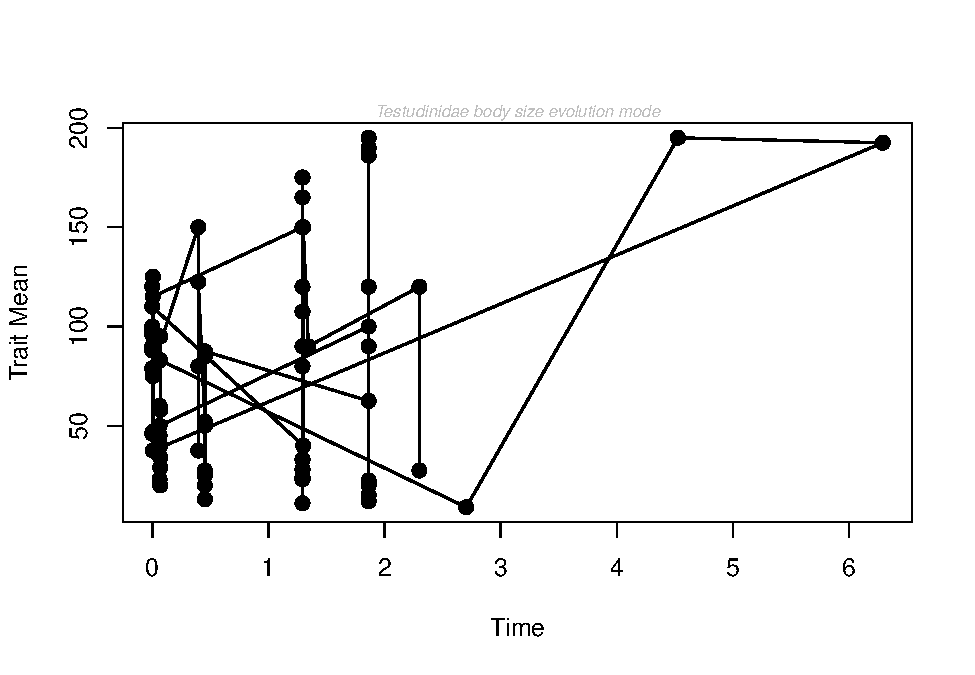
\includegraphics{tortoise_notes_files/figure-latex/unnamed-chunk-2-1.pdf}

This is the underlying data for Test1:

\begin{Shaded}
\begin{Highlighting}[]
\NormalTok{Test1}
\end{Highlighting}
\end{Shaded}

\begin{verbatim}
##       mm vv nn      tt
## 1  107.5  0  1 1.29350
## 2   24.0  0  1 1.29350
## 3   28.0  0  1 1.29350
## 4   23.0  0  1 1.29350
## 5  165.0  0  1 1.29350
## 6   80.0  0  1 1.29350
## 7  120.0  0  1 1.29350
## 8  175.0  0  1 1.29350
## 9   11.0  0  1 1.29350
## 10  90.0  0  1 1.29350
## 11  33.0  0  1 1.29350
## 12 150.0  0  1 1.29350
## 13 115.0  0  1 0.00585
## 14 125.0  0  1 0.00585
## 15  47.0  0  1 0.00585
## 16  75.0  0  1 0.00585
## 17  37.5  0  1 0.00585
## 18 192.5  0  1 6.28900
## 19 195.0  0  1 4.52600
## 20   9.0  0  1 2.70300
## 21  83.0  0  1 0.06885
## 22  95.0  0  1 0.06885
## 23  40.0  0  1 0.06885
## 24  58.0  0  1 0.06885
## 25  34.0  0  1 0.06885
## 26  29.0  0  1 0.06885
## 27  20.0  0  1 0.06885
## 28  23.0  0  1 0.06350
## 29  45.0  0  1 0.06350
## 30  60.0  0  1 0.06350
## 31  50.0  0  1 0.06300
## 32 100.0  0  1 1.86300
## 33 190.0  0  1 1.86300
## 34  22.0  0  1 1.86300
## 35 100.0  0  1 1.86300
## 36  90.0  0  1 1.86300
## 37 195.0  0  1 1.86300
## 38 120.0  0  1 1.86300
## 39  20.0  0  1 1.86300
## 40  12.0  0  1 1.86300
## 41  22.5  0  1 1.86300
## 42  15.0  0  1 1.86300
## 43 186.0  0  1 1.86300
## 44  62.5  0  1 1.86300
## 45  87.5  0  1 0.45350
## 46  85.0  0  1 0.45350
## 47  50.0  0  1 0.45350
## 48  20.0  0  1 0.45350
## 49  25.0  0  1 0.45350
## 50  13.0  0  1 0.45350
## 51  27.5  0  1 0.45350
## 52  52.0  0  1 0.45350
## 53 122.5  0  1 0.39635
## 54  80.0  0  1 0.39635
## 55  37.5  0  1 0.39635
## 56 150.0  0  1 0.39635
## 57  79.0  0  1 0.00000
## 58  98.0  0  1 0.00000
## 59  96.0  0  1 0.00000
## 60  88.0  0  1 0.00000
## 61  90.0  0  1 0.00000
## 62 100.0  0  1 0.00000
## 63  46.0  0  1 0.00000
## 64 100.0  0  1 0.00000
## 65 120.0  0  1 0.00000
## 66 110.0  0  1 0.00000
## 67  40.0  0  1 1.29985
## 68 150.0  0  1 1.29985
## 69  90.0  0  1 1.34400
## 70 120.0  0  1 2.30000
## 71  27.5  0  1 2.30000
\end{verbatim}

For the second plot, I averaged CL means across taxa for each time bin,
which leaves one data point per time bin, comprising all taxa within the
respective bin:

\begin{Shaded}
\begin{Highlighting}[]
\NormalTok{Test2 <-}\StringTok{ }\NormalTok{test %>%}
\StringTok{  }\KeywordTok{group_by}\NormalTok{(Age_mean) %>%}
\StringTok{  }\KeywordTok{summarise}\NormalTok{(}\DataTypeTok{mm =} \KeywordTok{mean}\NormalTok{(CL_mean), }\DataTypeTok{nn=}\KeywordTok{n}\NormalTok{(), }\DataTypeTok{vv=}\KeywordTok{var}\NormalTok{(CL_mean)) %>%}
\StringTok{  }\KeywordTok{mutate}\NormalTok{(}\DataTypeTok{tt=}\NormalTok{Age_mean) %>%}
\StringTok{  }\NormalTok{dplyr::}\KeywordTok{select}\NormalTok{(mm, vv, nn, tt)}

\CommentTok{# NA: column 2, rows 3, 10, 13, 14, 15}
\NormalTok{Test2[}\DecValTok{3}\NormalTok{,}\DecValTok{2}\NormalTok{] <-}\StringTok{ }\DecValTok{0}
\NormalTok{Test2[}\DecValTok{10}\NormalTok{,}\DecValTok{2}\NormalTok{] <-}\StringTok{ }\DecValTok{0}
\NormalTok{Test2[}\DecValTok{13}\NormalTok{,}\DecValTok{2}\NormalTok{] <-}\StringTok{ }\DecValTok{0}
\NormalTok{Test2[}\DecValTok{14}\NormalTok{,}\DecValTok{2}\NormalTok{] <-}\StringTok{ }\DecValTok{0}
\NormalTok{Test2[}\DecValTok{15}\NormalTok{,}\DecValTok{2}\NormalTok{] <-}\StringTok{ }\DecValTok{0}

\NormalTok{paleoTest2 <-}\KeywordTok{as.paleoTS}\NormalTok{(Test2$mm, Test2$vv, Test2$nn, Test2$tt, }\DataTypeTok{MM =} \OtherTok{NULL}\NormalTok{,}
                        \DataTypeTok{genpars =} \OtherTok{NULL}\NormalTok{, }\DataTypeTok{label =} \StringTok{"Testudinidae body size evolution mode"}\NormalTok{)}
\NormalTok{paleoTest2}
\end{Highlighting}
\end{Shaded}

\begin{verbatim}
## $mm
##  [1]  92.70000  79.90000  50.00000  42.66667  51.28571  97.50000  45.00000
##  [8]  83.87500  95.00000  90.00000  87.30769  73.75000   9.00000 195.00000
## [15] 192.50000
## 
## $vv
##  [1]  398.6778 1542.5500    0.0000  346.3333  810.5714 2429.1667  833.6429
##  [8] 3589.5511 6050.0000    0.0000 4816.0224 4278.1250    0.0000    0.0000
## [15]    0.0000
## 
## $nn
##  [1] 10  5  1  3  7  4  8 12  2  1 13  2  1  1  1
## 
## $tt
##  [1] 0.00000 0.00585 0.06300 0.06350 0.06885 0.39635 0.45350 1.29350
##  [9] 1.29985 1.34400 1.86300 2.30000 2.70300 4.52600 6.28900
## 
## $MM
## NULL
## 
## $genpars
## NULL
## 
## $label
## [1] "Testudinidae body size evolution mode"
## 
## $start.age
## NULL
## 
## $timeDir
## [1] "increasing"
## 
## attr(,"class")
## [1] "paleoTS"
\end{verbatim}

\begin{Shaded}
\begin{Highlighting}[]
\KeywordTok{plot}\NormalTok{(paleoTest2)}
\end{Highlighting}
\end{Shaded}

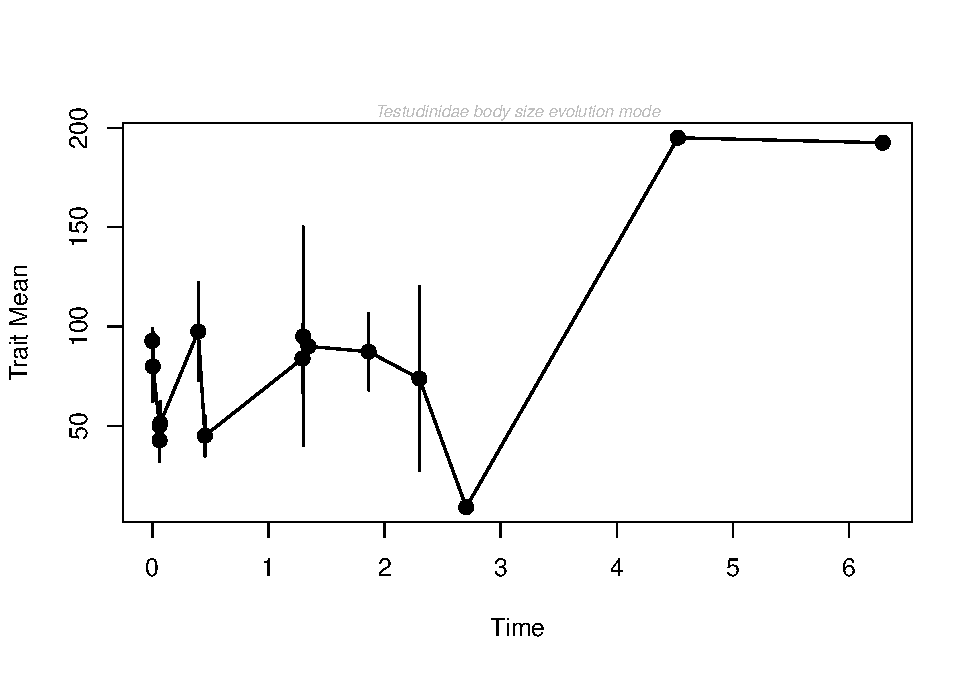
\includegraphics{tortoise_notes_files/figure-latex/unnamed-chunk-4-1.pdf}
Since ``real'' variances and sample sizes are available when pooling all
taxa, you can even fit models (as you should be able to in the end).
(when I remember correctly, the model with the highest Akaike.wt is the
best supported one, in this case this would be URW = random walk)

\begin{Shaded}
\begin{Highlighting}[]
\NormalTok{a=}\KeywordTok{fit3models}\NormalTok{(paleoTest2, }\DataTypeTok{silent=}\OtherTok{FALSE}\NormalTok{, }\DataTypeTok{method=}\StringTok{"AD"}\NormalTok{, }\DataTypeTok{pool=}\OtherTok{FALSE}\NormalTok{)   }\CommentTok{#not working with Test1, because no variances/sample sizes available, I guess}
\end{Highlighting}
\end{Shaded}

\begin{verbatim}
## 
## Comparing 3 models [n = 14, method = AD]
## 
##             logL K     AICc Akaike.wt
## GRW    -70.40398 2 145.8989     0.373
## URW    -71.26818 1 144.8697     0.625
## Stasis -75.70460 2 156.5001     0.002
\end{verbatim}

\begin{Shaded}
\begin{Highlighting}[]
\KeywordTok{str}\NormalTok{(a)}
\end{Highlighting}
\end{Shaded}

\begin{verbatim}
## 'data.frame':    3 obs. of  4 variables:
##  $ logL     : num  -70.4 -71.3 -75.7
##  $ K        : num  2 1 2
##  $ AICc     : num  146 145 157
##  $ Akaike.wt: num  0.373 0.625 0.002
\end{verbatim}

\begin{Shaded}
\begin{Highlighting}[]
\NormalTok{a$AICc[}\DecValTok{1}\NormalTok{] }\CommentTok{# not sure what this tells me...}
\end{Highlighting}
\end{Shaded}

\begin{verbatim}
## [1] 145.8989
\end{verbatim}

This is the underlying data for Test2:

\begin{Shaded}
\begin{Highlighting}[]
\NormalTok{Test2}
\end{Highlighting}
\end{Shaded}

\begin{verbatim}
## # A tibble: 15 × 4
##           mm        vv    nn      tt
##        <dbl>     <dbl> <int>   <dbl>
## 1   92.70000  398.6778    10 0.00000
## 2   79.90000 1542.5500     5 0.00585
## 3   50.00000    0.0000     1 0.06300
## 4   42.66667  346.3333     3 0.06350
## 5   51.28571  810.5714     7 0.06885
## 6   97.50000 2429.1667     4 0.39635
## 7   45.00000  833.6429     8 0.45350
## 8   83.87500 3589.5511    12 1.29350
## 9   95.00000 6050.0000     2 1.29985
## 10  90.00000    0.0000     1 1.34400
## 11  87.30769 4816.0224    13 1.86300
## 12  73.75000 4278.1250     2 2.30000
## 13   9.00000    0.0000     1 2.70300
## 14 195.00000    0.0000     1 4.52600
## 15 192.50000    0.0000     1 6.28900
\end{verbatim}

\subsection{TO DO:}\label{to-do}

\begin{itemize}
\item figure out if Checklist data is of any use (means? medians? sample size?) or see if authors can provide necessary data
\item do paleoTS analyses with FFB data set
\item read Hunt papers (see citations in Catalina's paper 2006, 2008, 2008, 2010; also 2015)
\item figure out how to implement phylogeny... well, figure out how to do paleoTS analyses with more than one taxon without pooling everything together (as in Test2)
\end{itemize}

\section{06.06.2017}\label{section-1}

Try paleoTS with some first real data. Here is the underlying data:

\begin{Shaded}
\begin{Highlighting}[]
\NormalTok{tidyCL<-}\KeywordTok{read.csv}\NormalTok{(}\StringTok{"tortoises_tidy.csv"}\NormalTok{, }\DataTypeTok{sep=}\StringTok{";"}\NormalTok{, }\DataTypeTok{header=}\OtherTok{TRUE}\NormalTok{)}
\NormalTok{tidyCL}
\end{Highlighting}
\end{Shaded}

\begin{verbatim}
##     Country Latitude Longitude
## 1       USA  37.6000 -120.6000
## 2       USA  37.6000 -120.8000
## 3       USA  37.6000 -120.6000
## 4       USA  38.6665  -76.5298
## 5       USA  37.2242 -100.4176
## 6       USA  42.0000  -97.0000
## 7       USA  34.9000 -101.6000
## 8       USA  27.7000  -82.5000
## 9       USA  42.7000 -100.0000
## 10      USA  29.7000  -82.6000
## 11      USA  29.6000  -82.4000
## 12   Greece  40.4046   22.8980
## 13   Greece  40.4046   22.8980
## 14  Germany  47.8356    8.7490
## 15  Germany  47.8356    8.7490
## 16  Germany  47.8356    8.7490
## 17  Germany  47.8356    8.7490
## 18  Germany  47.8356    8.7490
## 19  Germany  47.8356    8.7490
## 20  Germany  47.8356    8.7490
## 21  Germany  47.8356    8.7490
## 22  Germany  47.8356    8.7490
## 23 Mongolia  47.1000   93.1667
## 24 Mongolia  47.1000   93.1667
## 25      USA  37.0000 -100.0000
## 26      USA  37.0000 -100.0000
## 27   France  44.8120    0.2133
## 28   France  43.6000    1.4333
## 29  Georgia  41.3200   44.3500
## 30      USA  35.4000  -76.8000
## 31      USA  35.3000 -118.5000
## 32      USA  35.3000 -118.5000
## 33      USA  35.3000 -118.5000
## 34      USA  29.7000  -82.6000
## 35      USA  29.7000  -82.6000
## 36 Colombia   3.2000  -75.2000
## 37                NA        NA
##                                                                                                                                                                                                                                                                                                                                                                                                                                                                                                                                                                                                                                                                          Formation.Location.comment
## 1                                                                                                                                                                                                                                                                                                                                                                                                                                                                                                                                                                                                                                    Upper Mehrten Formation, Modesto Reservoir Member, Hemphillian
## 2                                                                                                                                                                                                                                                                                                                                                                                                                                                                                                                                                                                                                                                                 San Pablo Formation, Clarendonian
## 3                                                                                                                                                                                                                                                                                                                                                                                                                                                                                                                                                                                                                                    Upper Mehrten Formation, Modesto Reservoir Member, Hemphillian
## 4                                                                                                                                                                                                                                                                                                                                                                                                                                                                                                                                                                                                                         Shattuck zones 10+11, Plum Point Member (Plum Point B), Calvert Formation
## 5                                                                                                                                                                                                                                                                                                                                                                                                                                                                                                                                                                                                                                                                                     Rancholabrean
## 6                                                                                                                                                                                                                                                                                                                                                                                                                                                                                                                                                                                                                                                                                  Late Hemphillian
## 7                                                                                                                                                                                                                                                                                                                                                                                                                                                                                                                                                                                                                                                 poorly lithified, coarse-grained, brown sandstone
## 8                                                                                                                                                                                                                                                                                                                                                                                                                                                                                                                                                                                                                                                                           late early Irvingtonian
## 9                                                                                                                                                                                                                                                                                                                                                                                                                                                                                                                                              Blancan also known as: UNSM Sand Draw locality; Frick Prospecting Locality 277; Magill; Owl Pellet; UM-Neb. sites 1-66, 2-66, 2-67, 4-67, 5-67, 1-68
## 10                                                                                                                                                                                                                                                                                                                                                                                                                                                                                                                                                                                                                                                                                Alachua Formation
## 11                                                                                                                                                                                                                                                                                                                                                                                                                                                                                                                                                                                                                                                      Illinoian or Kansan according to Lynch 1965
## 12                                                                                                                                                                                                                                                                                                                                                                                                                                                                                                                                                                                                                                                                                  Gonia Formation
## 13                                                                                                                                                                                                                                                                                                                                                                                                                                                                                                                                                                                                                                                                                  Gonia Formation
## 14                                                                                                                                                                                                                                                                                                                                                                                                                                                                                                                                                                                                                                         pedogenic gypsum, red and yellow-mottled clays and marls
## 15                                                                                                                                                                                                                                                                                                                                                                                                                                                                                                                                                                                                                                         pedogenic gypsum, red and yellow-mottled clays and marls
## 16                                                                                                                                                                                                                                                                                                                                                                                                                                                                                                                                                                                                                                         pedogenic gypsum, red and yellow-mottled clays and marls
## 17                                                                                                                                                                                                                                                                                                                                                                                                                                                                                                                                                                                                                                         pedogenic gypsum, red and yellow-mottled clays and marls
## 18                                                                                                                                                                                                                                                                                                                                                                                                                                                                                                                                                                                                                                         pedogenic gypsum, red and yellow-mottled clays and marls
## 19                                                                                                                                                                                                                                                                                                                                                                                                                                                                                                                                                                                                                                         pedogenic gypsum, red and yellow-mottled clays and marls
## 20                                                                                                                                                                                                                                                                                                                                                                                                                                                                                                                                                                                                                                         pedogenic gypsum, red and yellow-mottled clays and marls
## 21                                                                                                                                                                                                                                                                                                                                                                                                                                                                                                                                                                                                                                         pedogenic gypsum, red and yellow-mottled clays and marls
## 22                                                                                                                                                                                                                                                                                                                                                                                                                                                                                                                                                                                                                                         pedogenic gypsum, red and yellow-mottled clays and marls
## 23                                                                                                                                                                                                                                                                                                                                                                                                                                                                                                                                                                                                                                                              160 km SW of Kobdo, Great Lake Area
## 24                                                                                                                                                                                                                                                                                                                                                                                                                                                                                                                                                                                                                                                              160 km SW of Kobdo, Great Lake Area
## 25                                                                                                                                                                                                                                                                                                                                                                                                                                                                                                                                                                                                                                                 XI Member of lower part of the Rexroad Formation
## 26                                                                                                                                                                                                                                                                                                                                                                                                                                                                                                                                                                                                                                                 XI Member of lower part of the Rexroad Formation
## 27                                                                                                                                                                                                                                                                                                                                                                                                                                                                                                                                                                                                                                                                   Molasse inférieur du Fronsadai
## 28                                                                                                                                                                                                                                                                                                                                                                                                                                                                                                                                                                                                                                                      Protaceratherium cf. minutum (Cuvier, 1822)
## 29                                                                                                                                                                                                                                                                                                                                                                                                                                                                                                                                                                                                                                                                                                -
## 30                                                                                                                                                                                                                                                                                                                                                                                                                                                                                                                                                                                                                                                                    Yorktown Formation muddy sand
## 31                                                                                                                                                                                                                                                                                                                                                                                                                                                                                                                                                                                                                                    Dove Spring Formation, Cerrotejonian, Clarendonian (CL1, CL2)
## 32                                                                                                                                                                                                                                                                                                                                                                                                                                                                                                                                                                                                                                     Dove Spring Formation, Montediablan, Clarendonian (CL2, CL3)
## 33                                                                                                                                                                                                                                                                                                                                                                                                                                                                                                                                                                                                                                     Dove Spring Formation, Montediablan, Clarendonian (CL2, CL3)
## 34 a sinkhole lake that then collapsed into a larger underground chamber earliest Hemmingfordian North American Land Mammal Age (NALMA) only Holman 1965, not Holman 2003: Leptodactylus abavus Holman, J. A. 1965. Quarterly Journal of the Florida Academy of Sciences 28(1):70-72, fig. 1. (Anura: Leptodactylidae; early Miocene). Holotype: UF 10201. Rana bucella, Holman, J. A. 1965. Quarterly Journal of the Florida Academy of Sciences 28(1):76-77, fig. 2. (Anura: Ranidae; early Miocene). Holotype: UF/FGS 6071. Rana miocenica Holman, J. A. 1965. Quarterly Journal of the Florida Academy of Sciences 28(1):74-76, fig. 2. (Anura: Ranidae; early Miocene). Holotype: UF/FGS 6069.
## 35 a sinkhole lake that then collapsed into a larger underground chamber earliest Hemmingfordian North American Land Mammal Age (NALMA) only Holman 1965, not Holman 2003: Leptodactylus abavus Holman, J. A. 1965. Quarterly Journal of the Florida Academy of Sciences 28(1):70-72, fig. 1. (Anura: Leptodactylidae; early Miocene). Holotype: UF 10201. Rana bucella, Holman, J. A. 1965. Quarterly Journal of the Florida Academy of Sciences 28(1):76-77, fig. 2. (Anura: Ranidae; early Miocene). Holotype: UF/FGS 6071. Rana miocenica Holman, J. A. 1965. Quarterly Journal of the Florida Academy of Sciences 28(1):74-76, fig. 2. (Anura: Ranidae; early Miocene). Holotype: UF/FGS 6069.
## 36                                                                                                                                                                                                                                                                                                                                                                                                                                                                                                                                                                                                                                                         Honda group, Cerbatana gravels and clays
## 37                                                                                                                                                                                                                                                                                                                                                                                                                                                                                                                                                                                                                                                                                                 
##     MAmin  Mamax          Genus       Species                        Taxon
## 1   5.000  6.000 Hesperotestudo    orthopygia    Hesperotestudo orthopygia
## 2   9.000 10.000 Hesperotestudo           sp.           Hesperotestudo sp.
## 3   5.000  6.000 Hesperotestudo    orthopygia    Hesperotestudo orthopygia
## 4  15.000 15.800     Floridemys         hurdi             Floridemys hurdi
## 5   0.300  0.300 Hesperotestudo     equicomes     Hesperotestudo equicomes
## 6   4.800  5.200     Geochelone           sp.               Geochelone sp.
## 7   1.800  3.600       Gopherus   canyonensis         Gopherus canyonensis
## 8   1.000  1.500 Hesperotestudo crassiscutata Hesperotestudo crassiscutata
## 9   3.000  3.000 Hesperotestudo      oelrichi      Hesperotestudo oelrichi
## 10 10.900 11.000 Hesperotestudo        alleni        Hesperotestudo alleni
## 11  0.012  0.126 Hesperotestudo        incisa        Hesperotestudo incisa
## 12  2.600  5.300   Titanochelon   bacharidisi     Titanochelon bacharidisi
## 13  2.600  5.300   Titanochelon   bacharidisi     Titanochelon bacharidisi
## 14 13.000 13.000   Paleotestudo       antiqua         Paleotestudo antiqua
## 15 13.000 13.000   Paleotestudo       antiqua         Paleotestudo antiqua
## 16 13.000 13.000   Paleotestudo       antiqua         Paleotestudo antiqua
## 17 13.000 13.000   Paleotestudo       antiqua         Paleotestudo antiqua
## 18 13.000 13.000   Paleotestudo       antiqua         Paleotestudo antiqua
## 19 13.000 13.000   Paleotestudo       antiqua         Paleotestudo antiqua
## 20 13.000 13.000   Paleotestudo       antiqua         Paleotestudo antiqua
## 21 13.000 13.000   Paleotestudo       antiqua         Paleotestudo antiqua
## 22 13.000 13.000   Paleotestudo       antiqua         Paleotestudo antiqua
## 23  2.600  5.300      Ergilemys    oskarkuhni         Ergilemys oskarkuhni
## 24  2.600  5.300      Ergilemys    oskarkuhni         Ergilemys oskarkuhni
## 25  3.000  3.000 Hesperotestudo        riggsi        Hesperotestudo riggsi
## 26  3.000  3.000 Hesperotestudo        riggsi        Hesperotestudo riggsi
## 27 33.900 34.000   Cheirogaster       maurini         Cheirogaster maurini
## 28 23.030 23.200      Ergilemys       bruneti            Ergilemys bruneti
## 29  1.770  1.770        Testudo        graeca               Testudo graeca
## 30  4.000  5.000     Geochelone           sp.               Geochelone sp.
## 31 11.200 12.500       Gopherus         ? sp.               Gopherus ? sp.
## 32  9.000 11.200     Geochelone           sp.               Geochelone sp.
## 33  9.000 11.200       Gopherus         ? sp.               Gopherus ? sp.
## 34 18.000 19.000     Geochelone     tedwhitei         Geochelone tedwhitei
## 35 18.000 19.000     Geochelone     tedwhitei         Geochelone tedwhitei
## 36  6.000 11.000     Geochelone      hesterna          Geochelone hesterna
## 37     NA     NA                                                          
##      CL     PL
## 1  1200     NA
## 2  1200     NA
## 3    NA  620.0
## 4    NA     NA
## 5    NA     NA
## 6    NA  160.0
## 7    NA  805.0
## 8    NA  510.0
## 9    NA  258.0
## 10   NA  219.0
## 11   NA  211.6
## 12 1196 1150.0
## 13 1164 1120.0
## 14  185     NA
## 15  229     NA
## 16  220     NA
## 17  195     NA
## 18  206     NA
## 19  196     NA
## 20   NA  102.0
## 21  150     NA
## 22  145     NA
## 23   NA  180.0
## 24  220     NA
## 25  176  189.0
## 26  185     NA
## 27  400     NA
## 28  400     NA
## 29  195     NA
## 30  880  700.0
## 31  500     NA
## 32  500     NA
## 33  500     NA
## 34  370     NA
## 35   NA  400.0
## 36  278     NA
## 37   NA     NA
##                                                                                                               verbal
## 1                                                                                                               <NA>
## 2                                                        very large (comparable to specimens from Mehrten Formation)
## 3                                                                                                               <NA>
## 4                                                                            smaller than Hesperotestudo or Gopherus
## 5                                                      medium to lage-sized Hesperotestudo, smaller than G. oelrichi
## 6                                                                                                               <NA>
## 7                                                                                                               <NA>
## 8                                                                              small (subgenus Hesperotestudo) lines
## 9                                  G. oelrichi is among the largest of the Geochelone (Hesperotestudo) turgida group
## 10                                                                                                              <NA>
## 11                                                                                                              <NA>
## 12                                                                                                              <NA>
## 13                                                                                                          subadult
## 14                                                                                                              <NA>
## 15                                                                                                              <NA>
## 16                                                                                                              <NA>
## 17                                                                                                              <NA>
## 18                                                                                                              <NA>
## 19                                                                                                        incomplete
## 20                                                                                                              <NA>
## 21                                                                                                              <NA>
## 22                                                                                                              <NA>
## 23                                                                                                              <NA>
## 24                                                                                                              <NA>
## 25                Holotype KUMVP 6789: CL: 176 mm(, C width: 155 mm, C height: 85 mm), PL: 189 mm(, P width: 140 mm)
## 26                                                                      Paratype KUMVP 6790: CL: 185 mm(, CW 165 mm)
## 27                                                                                                    close to 40 cm
## 28                                                                                                              <NA>
## 29                                                                                                              <NA>
## 30                                                                                                             large
## 31 Tortoises (Geochelone sp. and ?Gopherus sp. with carapaces up to 0.5 m in length are found throughout the section
## 32 Tortoises (Geochelone sp. and ?Gopherus sp. with carapaces up to 0.5 m in length are found throughout the section
## 33 Tortoises (Geochelone sp. and ?Gopherus sp. with carapaces up to 0.5 m in length are found throughout the section
## 34                                                                         CL: 370 mm, CW: 300 mm, CH approx. 150 mm
## 35                                                                     several specimens: not exceeding 400 mm in PL
## 36                                                                                                              <NA>
## 37                                                                                                                  
##    estimated..e..from.verbal.description..ev..from.plastron..ep..or.measured..m..measured.from.figure..mf..
## 1                                                                                                         e
## 2                                                                                                        ev
## 3                                                                                                         e
## 4                                                                                                        ev
## 5                                                                                                        ev
## 6                                                                                                         e
## 7                                                                                                         m
## 8                                                                                                         m
## 9                                                                                                         m
## 10                                                                                                        m
## 11                                                                                                        m
## 12                                                                                                        m
## 13                                                                                                        m
## 14                                                                                                       mf
## 15                                                                                                       mf
## 16                                                                                                       mf
## 17                                                                                                       mf
## 18                                                                                                       mf
## 19                                                                                                       mf
## 20                                                                                                       mf
## 21                                                                                                       mf
## 22                                                                                                       mf
## 23                                                                                                        m
## 24                                                                                                        m
## 25                                                                                                        m
## 26                                                                                                        m
## 27                                                                                                        m
## 28                                                                                                        m
## 29                                                                                                       mf
## 30                                                                                                        m
## 31                                                                                                        m
## 32                                                                                                        m
## 33                                                                                                        m
## 34                                                                                                        m
## 35                                                                                                        m
## 36                                                                                                        m
## 37
\end{verbatim}

Prepare data for conversion to paleoTS-object:

\begin{Shaded}
\begin{Highlighting}[]
\NormalTok{TidyCL <-}\StringTok{ }\NormalTok{tidyCL %>%}
\StringTok{  }\KeywordTok{select}\NormalTok{(MAmin, Mamax, CL) %>%}
\StringTok{  }\KeywordTok{filter}\NormalTok{(CL !=}\StringTok{ "NA"}\NormalTok{) %>%}
\StringTok{  }\KeywordTok{mutate}\NormalTok{(}\DataTypeTok{tt=} \NormalTok{(MAmin+Mamax)/}\DecValTok{2}\NormalTok{) %>%}\StringTok{ }\CommentTok{# create mean age}
\StringTok{  }\KeywordTok{group_by}\NormalTok{(tt) %>%}\StringTok{ }\CommentTok{#create time bins}
\StringTok{  }\KeywordTok{summarise}\NormalTok{(}\DataTypeTok{mm=}\KeywordTok{mean}\NormalTok{(CL), }\DataTypeTok{vv=}\KeywordTok{var}\NormalTok{(CL), }\DataTypeTok{nn=}\KeywordTok{n}\NormalTok{()) }\CommentTok{#create means etc. for each time bin }

\NormalTok{TidyCL[}\KeywordTok{is.na}\NormalTok{(TidyCL)]<-}\DecValTok{0} \CommentTok{#subset NAs with O for }

\NormalTok{TidyCL}
\end{Highlighting}
\end{Shaded}

\begin{verbatim}
## # A tibble: 13 × 4
##        tt      mm          vv    nn
##     <dbl>   <dbl>       <dbl> <int>
## 1   1.770  195.00      0.0000     1
## 2   3.000  180.50     40.5000     2
## 3   3.950  860.00 307456.0000     3
## 4   4.500  880.00      0.0000     1
## 5   5.500 1200.00      0.0000     1
## 6   8.500  278.00      0.0000     1
## 7   9.500 1200.00      0.0000     1
## 8  10.100  500.00      0.0000     2
## 9  11.850  500.00      0.0000     1
## 10 13.000  190.75    911.9286     8
## 11 18.500  370.00      0.0000     1
## 12 23.115  400.00      0.0000     1
## 13 33.950  400.00      0.0000     1
\end{verbatim}

\begin{Shaded}
\begin{Highlighting}[]
\NormalTok{bins <-}\StringTok{ }\NormalTok{tidyCL %>%}
\CommentTok{#  select(MAmin, Mamax, CL) %>%}
\StringTok{  }\KeywordTok{filter}\NormalTok{(CL !=}\StringTok{ "NA"}\NormalTok{) %>%}
\StringTok{  }\KeywordTok{mutate}\NormalTok{(}\DataTypeTok{tt=} \NormalTok{(MAmin+Mamax)/}\DecValTok{2}\NormalTok{) %>%}\StringTok{ }\CommentTok{# create mean age}
\StringTok{  }\KeywordTok{group_by}\NormalTok{(tt)}

\NormalTok{bins}
\end{Highlighting}
\end{Shaded}

\begin{verbatim}
## Source: local data frame [24 x 14]
## Groups: tt [13]
## 
##    Country Latitude Longitude
##     <fctr>    <dbl>     <dbl>
## 1      USA  37.6000  -120.600
## 2      USA  37.6000  -120.800
## 3   Greece  40.4046    22.898
## 4   Greece  40.4046    22.898
## 5  Germany  47.8356     8.749
## 6  Germany  47.8356     8.749
## 7  Germany  47.8356     8.749
## 8  Germany  47.8356     8.749
## 9  Germany  47.8356     8.749
## 10 Germany  47.8356     8.749
## # ... with 14 more rows, and 11 more variables:
## #   Formation.Location.comment <fctr>, MAmin <dbl>, Mamax <dbl>,
## #   Genus <fctr>, Species <fctr>, Taxon <fctr>, CL <int>, PL <dbl>,
## #   verbal <fctr>,
## #   estimated..e..from.verbal.description..ev..from.plastron..ep..or.measured..m..measured.from.figure..mf.. <fctr>,
## #   tt <dbl>
\end{verbatim}

\begin{Shaded}
\begin{Highlighting}[]
\KeywordTok{library}\NormalTok{(paleoTS)}
\NormalTok{paleoTidyCL <-}\KeywordTok{as.paleoTS}\NormalTok{(TidyCL$mm, TidyCL$vv, TidyCL$nn, TidyCL$tt, }\DataTypeTok{MM =} \OtherTok{NULL}\NormalTok{, }\DataTypeTok{genpars =} \OtherTok{NULL}\NormalTok{, }\DataTypeTok{label =} \StringTok{"Testudinidae body size evolution mode"}\NormalTok{)}
\NormalTok{paleoTidyCL}
\end{Highlighting}
\end{Shaded}

\begin{verbatim}
## $mm
##  [1]  195.00  180.50  860.00  880.00 1200.00  278.00 1200.00  500.00
##  [9]  500.00  190.75  370.00  400.00  400.00
## 
## $vv
##  [1]      0.0000     40.5000 307456.0000      0.0000      0.0000
##  [6]      0.0000      0.0000      0.0000      0.0000    911.9286
## [11]      0.0000      0.0000      0.0000
## 
## $nn
##  [1] 1 2 3 1 1 1 1 2 1 8 1 1 1
## 
## $tt
##  [1]  0.000  1.230  2.180  2.730  3.730  6.730  7.730  8.330 10.080 11.230
## [11] 16.730 21.345 32.180
## 
## $MM
## NULL
## 
## $genpars
## NULL
## 
## $label
## [1] "Testudinidae body size evolution mode"
## 
## $start.age
## [1] 1.77
## 
## $timeDir
## [1] "increasing"
## 
## attr(,"class")
## [1] "paleoTS"
\end{verbatim}

\begin{Shaded}
\begin{Highlighting}[]
\KeywordTok{plot}\NormalTok{(paleoTidyCL)}
\end{Highlighting}
\end{Shaded}

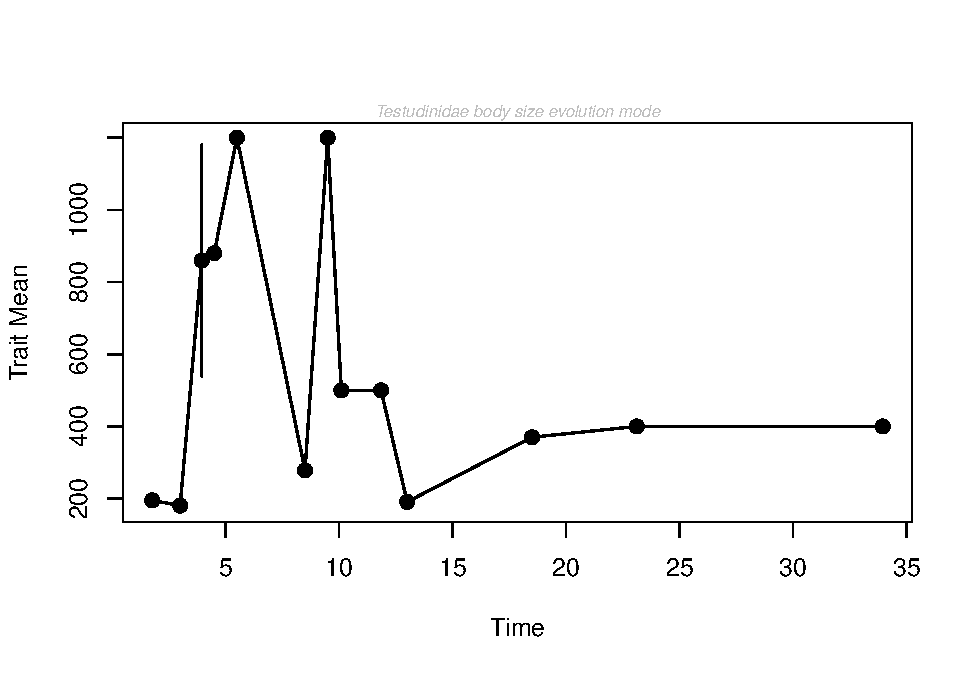
\includegraphics{tortoise_notes_files/figure-latex/unnamed-chunk-9-1.pdf}

\begin{Shaded}
\begin{Highlighting}[]
\KeywordTok{fit3models}\NormalTok{(paleoTidyCL, }\DataTypeTok{silent=}\OtherTok{FALSE}\NormalTok{, }\DataTypeTok{method=}\StringTok{"AD"}\NormalTok{, }\DataTypeTok{pool=}\OtherTok{FALSE}\NormalTok{)   }\CommentTok{#not working with Test1, because no variances/sample sizes available, I guess}
\end{Highlighting}
\end{Shaded}

\begin{verbatim}
## 
## Comparing 3 models [n = 12, method = AD]
## 
##              logL K     AICc Akaike.wt
## GRW     -94.17747 2 193.6883     0.001
## URW    -104.37703 1 211.1541     0.000
## Stasis  -87.43872 2 180.2108     0.999
\end{verbatim}

\subsection{TO DO:}\label{to-do-1}

\begin{itemize}
\tightlist
\item
  map localities with differing colors for: CL available, CL
  extrapolated (from PL or figures), CL missing
\item
  complete data set!
\item
  get missing refences/make list of missing references
\end{itemize}

This is an \href{http://rmarkdown.rstudio.com}{R Markdown} Notebook.
When you execute code within the notebook, the results appear beneath
the code.

Try executing this chunk by clicking the \emph{Run} button within the
chunk or by placing your cursor inside it and pressing
\emph{Ctrl+Shift+Enter}.

Add a new chunk by clicking the \emph{Insert Chunk} button on the
toolbar or by pressing \emph{Ctrl+Alt+I}.

When you save the notebook, an HTML file containing the code and output
will be saved alongside it (click the \emph{Preview} button or press
\emph{Ctrl+Shift+K} to preview the HTML file).


\end{document}
